% Options for packages loaded elsewhere
\PassOptionsToPackage{unicode}{hyperref}
\PassOptionsToPackage{hyphens}{url}
%
\documentclass[
  ignorenonframetext,
]{beamer}
\usepackage{pgfpages}
\setbeamertemplate{caption}[numbered]
\setbeamertemplate{caption label separator}{: }
\setbeamercolor{caption name}{fg=normal text.fg}
\beamertemplatenavigationsymbolsempty
% Prevent slide breaks in the middle of a paragraph
\widowpenalties 1 10000
\raggedbottom
\setbeamertemplate{part page}{
  \centering
  \begin{beamercolorbox}[sep=16pt,center]{part title}
    \usebeamerfont{part title}\insertpart\par
  \end{beamercolorbox}
}
\setbeamertemplate{section page}{
  \centering
  \begin{beamercolorbox}[sep=12pt,center]{part title}
    \usebeamerfont{section title}\insertsection\par
  \end{beamercolorbox}
}
\setbeamertemplate{subsection page}{
  \centering
  \begin{beamercolorbox}[sep=8pt,center]{part title}
    \usebeamerfont{subsection title}\insertsubsection\par
  \end{beamercolorbox}
}
\AtBeginPart{
  \frame{\partpage}
}
\AtBeginSection{
  \ifbibliography
  \else
    \frame{\sectionpage}
  \fi
}
\AtBeginSubsection{
  \frame{\subsectionpage}
}
\usepackage{amsmath,amssymb}
\usepackage{lmodern}
\usepackage{ifxetex,ifluatex}
\ifnum 0\ifxetex 1\fi\ifluatex 1\fi=0 % if pdftex
  \usepackage[T1]{fontenc}
  \usepackage[utf8]{inputenc}
  \usepackage{textcomp} % provide euro and other symbols
\else % if luatex or xetex
  \usepackage{unicode-math}
  \defaultfontfeatures{Scale=MatchLowercase}
  \defaultfontfeatures[\rmfamily]{Ligatures=TeX,Scale=1}
  \setmainfont[BoldFont = SF Pro Rounded Semibold]{SF Pro Rounded}
  \setmathfont[]{STIX Two Math}
\fi
\usefonttheme{serif} % use mainfont rather than sansfont for slide text
% Use upquote if available, for straight quotes in verbatim environments
\IfFileExists{upquote.sty}{\usepackage{upquote}}{}
\IfFileExists{microtype.sty}{% use microtype if available
  \usepackage[]{microtype}
  \UseMicrotypeSet[protrusion]{basicmath} % disable protrusion for tt fonts
}{}
\makeatletter
\@ifundefined{KOMAClassName}{% if non-KOMA class
  \IfFileExists{parskip.sty}{%
    \usepackage{parskip}
  }{% else
    \setlength{\parindent}{0pt}
    \setlength{\parskip}{6pt plus 2pt minus 1pt}}
}{% if KOMA class
  \KOMAoptions{parskip=half}}
\makeatother
\usepackage{xcolor}
\IfFileExists{xurl.sty}{\usepackage{xurl}}{} % add URL line breaks if available
\IfFileExists{bookmark.sty}{\usepackage{bookmark}}{\usepackage{hyperref}}
\hypersetup{
  pdftitle={305 Lecture 5.5 - Strategies 2: Working Forwards},
  pdfauthor={Brian Weatherson},
  hidelinks,
  pdfcreator={LaTeX via pandoc}}
\urlstyle{same} % disable monospaced font for URLs
\newif\ifbibliography
\usepackage{graphicx}
\makeatletter
\def\maxwidth{\ifdim\Gin@nat@width>\linewidth\linewidth\else\Gin@nat@width\fi}
\def\maxheight{\ifdim\Gin@nat@height>\textheight\textheight\else\Gin@nat@height\fi}
\makeatother
% Scale images if necessary, so that they will not overflow the page
% margins by default, and it is still possible to overwrite the defaults
% using explicit options in \includegraphics[width, height, ...]{}
\setkeys{Gin}{width=\maxwidth,height=\maxheight,keepaspectratio}
% Set default figure placement to htbp
\makeatletter
\def\fps@figure{htbp}
\makeatother
\setlength{\emergencystretch}{3em} % prevent overfull lines
\providecommand{\tightlist}{%
  \setlength{\itemsep}{0pt}\setlength{\parskip}{0pt}}
\setcounter{secnumdepth}{-\maxdimen} % remove section numbering
\let\Tiny=\tiny

 \setbeamertemplate{navigation symbols}{} 

% \usetheme{Madrid}
 \usetheme[numbering=none, progressbar=foot]{metropolis}
 \usecolortheme{wolverine}
 \usepackage{color}
 \usepackage{MnSymbol}
% \usepackage{movie15}

\usepackage{amssymb}% http://ctan.org/pkg/amssymb
\usepackage{pifont}% http://ctan.org/pkg/pifont
\newcommand{\cmark}{\ding{51}}%
\newcommand{\xmark}{\ding{55}}%

\DeclareSymbolFont{symbolsC}{U}{txsyc}{m}{n}
\DeclareMathSymbol{\boxright}{\mathrel}{symbolsC}{128}
\DeclareMathAlphabet{\mathpzc}{OT1}{pzc}{m}{it}

\usepackage{tikz-qtree}
% \usepackage{markdown}
%\RequirePackage{bussproofs}
\usetikzlibrary{arrows.meta}
\RequirePackage[tableaux]{prooftrees}
\forestset{line numbering, close with = x}
% Allow for easy commas inside trees
\renewcommand{\,}{\text{, }}


\usepackage{tabulary}

\usepackage{open-logic-config}

\setlength{\parskip}{1ex plus 0.5ex minus 0.2ex}

\AtBeginSection[]
{
\begin{frame}
	\Huge{\color{darkblue} \insertsection}
\end{frame}
}

\renewenvironment*{quote}	
	{\list{}{\rightmargin   \leftmargin} \item } 	
	{\endlist }

\definecolor{darkgreen}{rgb}{0,0.7,0}
\definecolor{darkblue}{rgb}{0,0,0.8}

\newcommand{\starttab}{\begin{center}
\vspace{6pt}
\begin{tabular}}

\newcommand{\stoptab}{\end{tabular}
\vspace{6pt}
\end{center}
\noindent}


\newcommand{\sif}{\rightarrow}
\newcommand{\siff}{\leftrightarrow}
\newcommand{\EF}{\end{frame}}


\newcommand{\TreeStart}[1]{
%\end{frame}
\begin{frame}
\begin{center}
\begin{tikzpicture}[scale=#1]
\tikzset{every tree node/.style={align=center,anchor=north}}
%\Tree
}

\newcommand{\TreeEnd}{
\end{tikzpicture}
%\end{center}
}

\newcommand{\DisplayArg}[2]{
\begin{enumerate}
{#1}
\end{enumerate}
\vspace{-6pt}
\hrulefill

%\hspace{14pt} #2
%{\addtolength{\leftskip}{14pt} #2}
\begin{quote}
{\normalfont #2}
\end{quote}
\vspace{12pt}
}

\newenvironment{ProofTree}[1][1]{
\begin{center}
\begin{tikzpicture}[scale=#1]
\tikzset{every tree node/.style={align=center,anchor=south}}
}
{
\end{tikzpicture}
\end{center}
}

\newcommand{\TreeFrame}[2]{
\begin{columns}[c]
\column{0.5\textwidth}
\begin{center}
\begin{prooftree}{}
#1
\end{prooftree}
\end{center}
\column{0.45\textwidth}
%\begin{markdown}
#2
%\end{markdown}
\end{columns}
}

\newcommand{\ScaledTreeFrame}[3]{
\begin{columns}[c]
\column{0.5\textwidth}
\begin{center}
\scalebox{#1}{
\begin{prooftree}{}
#2
\end{prooftree}
}
\end{center}
\column{0.45\textwidth}
%\begin{markdown}
#3
%\end{markdown}
\end{columns}
}

\usepackage[bb=boondox]{mathalfa}
\DeclareMathAlphabet{\mathbx}{U}{BOONDOX-ds}{m}{n}
\SetMathAlphabet{\mathbx}{bold}{U}{BOONDOX-ds}{b}{n}
\DeclareMathAlphabet{\mathbbx} {U}{BOONDOX-ds}{b}{n}


\newenvironment{oltableau}{\center\tableau{}} %wff format={anchor = base west}}}
       {\endtableau\endcenter}
       
\newcommand{\formula}[1]{$#1$}

\usepackage{tabulary}
\usepackage{booktabs}

\def\begincols{\begin{columns}}
\def\begincol{\begin{column}}
\def\endcol{\end{column}}
\def\endcols{\end{columns}}

\usepackage[italic]{mathastext}
\usepackage{nicefrac}

\definecolor{mygreen}{RGB}{0, 100, 0}
\definecolor{mypink2}{RGB}{219, 48, 122}
\definecolor{dodgerblue}{RGB}{30,144,255}

%\def\True{\textcolor{dodgerblue}{\text{T}}}
%\def\False{\textcolor{red}{\text{F}}}

\def\True{\mathbb{T}}
\def\False{\mathbb{F}}

% This is because arguments didn't have enough space after them
\usepackage{etoolbox}
\AfterEndEnvironment{description}{\vspace{9pt}}
\AfterEndEnvironment{oltableau}{\vspace{9pt}}
\BeforeBeginEnvironment{oltableau}{\vspace{9pt}}
\AfterEndEnvironment{center}{\vspace{12pt}}
\BeforeBeginEnvironment{tabular}{\vspace{9pt}}

\setlength\heavyrulewidth{0pt}
\setlength\lightrulewidth{0pt}

%\def\toprule{}
%\def\bottomrule{}
%\def\midrule{}

\setbeamertemplate{caption}{\raggedright\insertcaption}

\ifluatex
  \usepackage{selnolig}  % disable illegal ligatures
\fi

\title{305 Lecture 5.5 - Strategies 2: Working Forwards}
\author{Brian Weatherson}
\date{}

\begin{document}
\frame{\titlepage}

\begin{frame}{Plan}
\protect\hypertarget{plan}{}
This lecture discusses strategies for constructing proofs that involve
working forwards.
\end{frame}

\begin{frame}{Associated Reading}
\protect\hypertarget{associated-reading}{}
forall x, section 17.2.
\end{frame}

\begin{frame}{Working Forwards}
\protect\hypertarget{working-forwards}{}
Big Idea: Plan to use the Elimination rules on the connectives in the
premises.
\end{frame}

\begin{frame}{Simple Illustration: And}
\protect\hypertarget{simple-illustration-and}{}
When one of the premises is of the form \(X \wedge y\), you'll almost
certainly need to apply \(\wedge\)E to get \(X\) and \(Y\).
\end{frame}

\begin{frame}{Slightly Trickier: If}
\protect\hypertarget{slightly-trickier-if}{}
\begin{itemize}[<+->]
\tightlist
\item
  When one of the premises is of the form \(X \rightarrow Y\), you'll
  almost certainly need to apply \(\rightarrow\)E.
\item
  And that means you'll need \(X\).
\item
  But in practice it's hard to tell in advance whether you'll prove
  \(X\), or have it as the start of a subproof, or something else.
\end{itemize}
\end{frame}

\begin{frame}{Working forward from Or}
\protect\hypertarget{working-forward-from-or}{}
When one of the premises is \(X \vee Y\) there is a clear(ish) strategy.

\begin{enumerate}
\tightlist
\item
  Find a target conclusion \(C\).
\item
  Do a subproof from \(X\) to \(C\).
\item
  Do a subproof from \(Y\) to \(C\).
\item
  Conclude \(C\) by \(\vee\)E.
\end{enumerate}
\end{frame}

\begin{frame}{Working forward from Or}
\protect\hypertarget{working-forward-from-or-1}{}
Why clear-ish?

\begin{itemize}
\tightlist
\item
  Because it isn't always true that the target here should be the
  conclusion of the whole argument.
\item
  Sometimes it is optimal to do a step or two of working backwards
  first.
\item
  But if you want a simple rule to go by, the best is to do what's on
  the previous slide with \(C\) as the conclusion of the whole argument.
\end{itemize}
\end{frame}

\begin{frame}{\(A \vee B, B \rightarrow C \vdash A \vee C\)}
\protect\hypertarget{a-vee-b-b-rightarrow-c-vdash-a-vee-c}{}
\begin{figure}
\centering
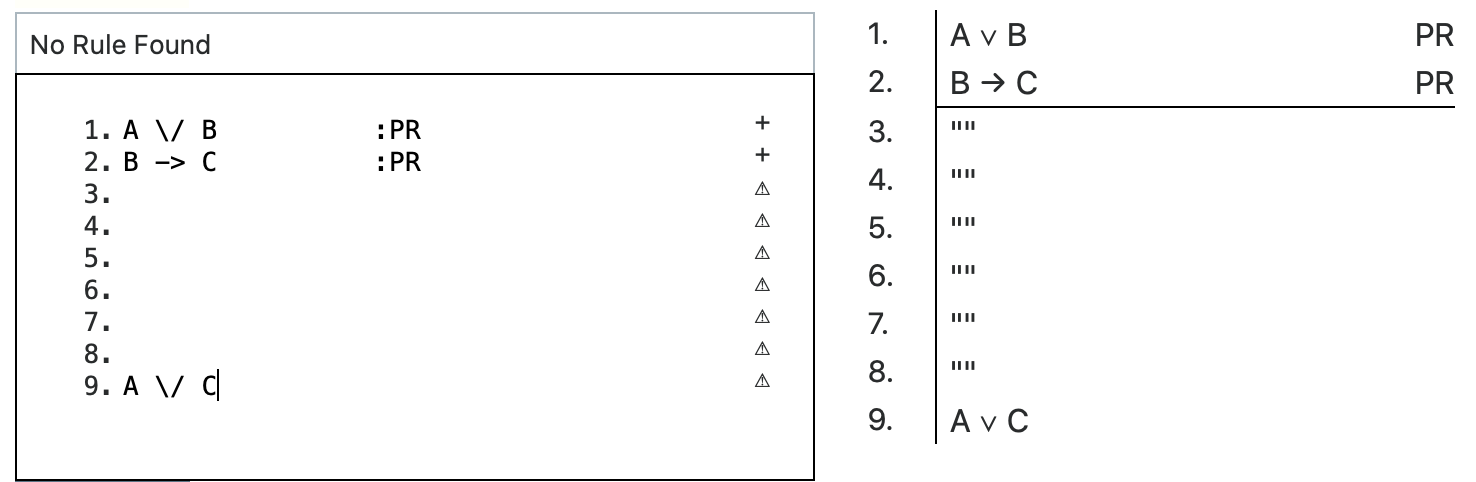
\includegraphics[width=\textwidth,height=0.75\textheight]{5_5a.png}
\caption{Write Out Premises and Conclusion}
\end{figure}
\end{frame}

\begin{frame}{\(A \vee B, B \rightarrow C \vdash A \vee C\)}
\protect\hypertarget{a-vee-b-b-rightarrow-c-vdash-a-vee-c-1}{}
\begin{figure}
\centering
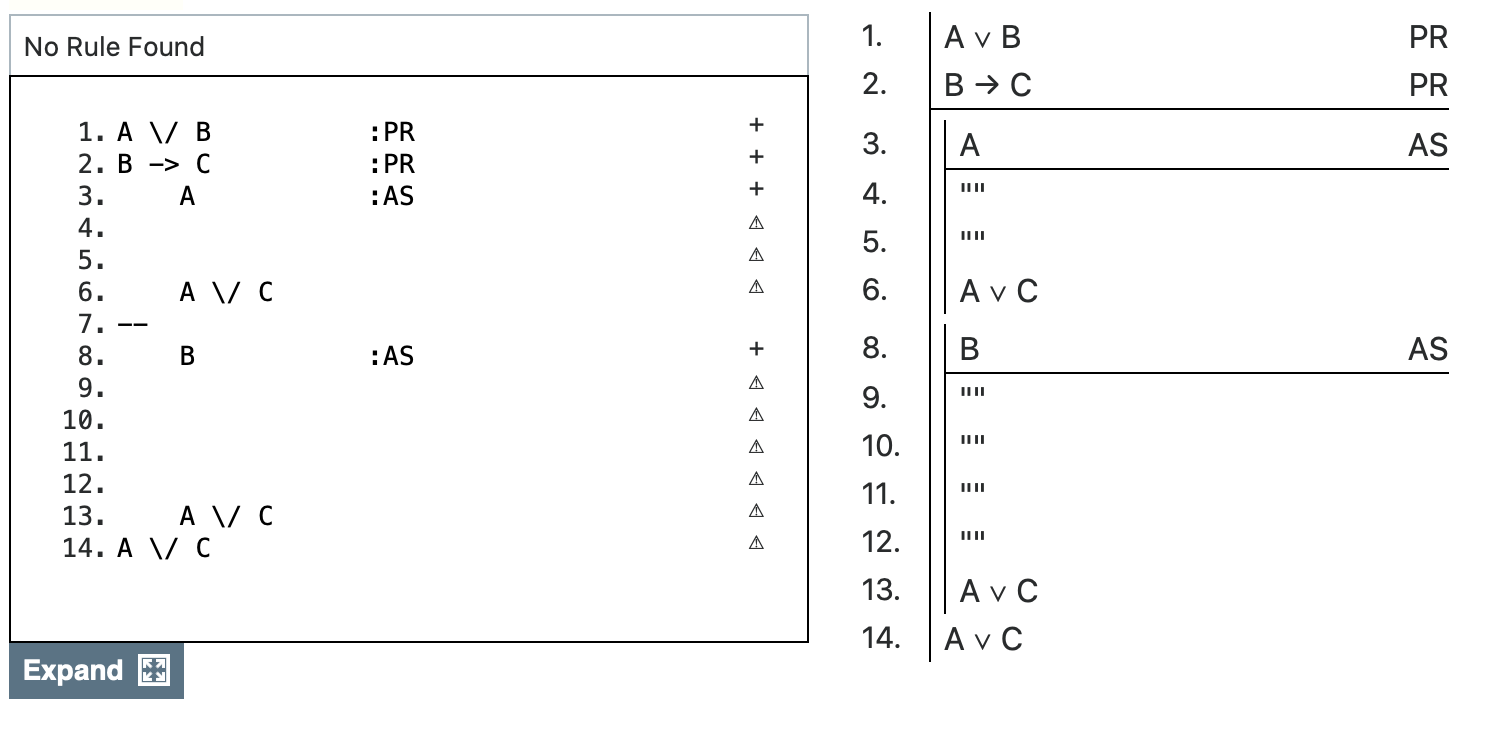
\includegraphics[width=\textwidth,height=0.75\textheight]{5_5b.png}
\caption{Set Up \(\vee\)E}
\end{figure}
\end{frame}

\begin{frame}{\(A \vee B, B \rightarrow C \vdash A \vee C\)}
\protect\hypertarget{a-vee-b-b-rightarrow-c-vdash-a-vee-c-2}{}
\begin{figure}
\centering
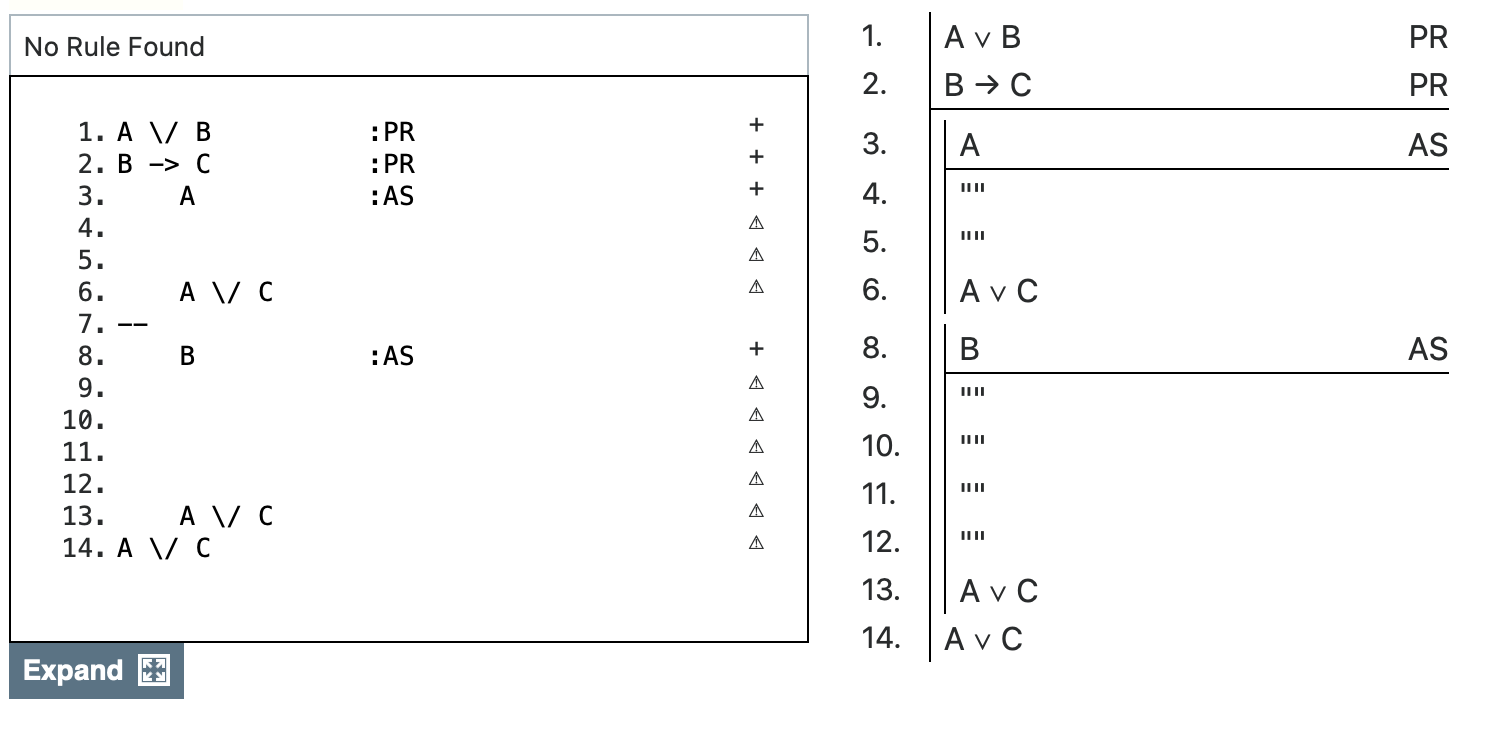
\includegraphics[width=\textwidth,height=0.75\textheight]{5_5b.png}
\caption{Note what happens on line 7}
\end{figure}
\end{frame}

\begin{frame}{\(A \vee B, B \rightarrow C \vdash A \vee C\)}
\protect\hypertarget{a-vee-b-b-rightarrow-c-vdash-a-vee-c-3}{}
\begin{figure}
\centering
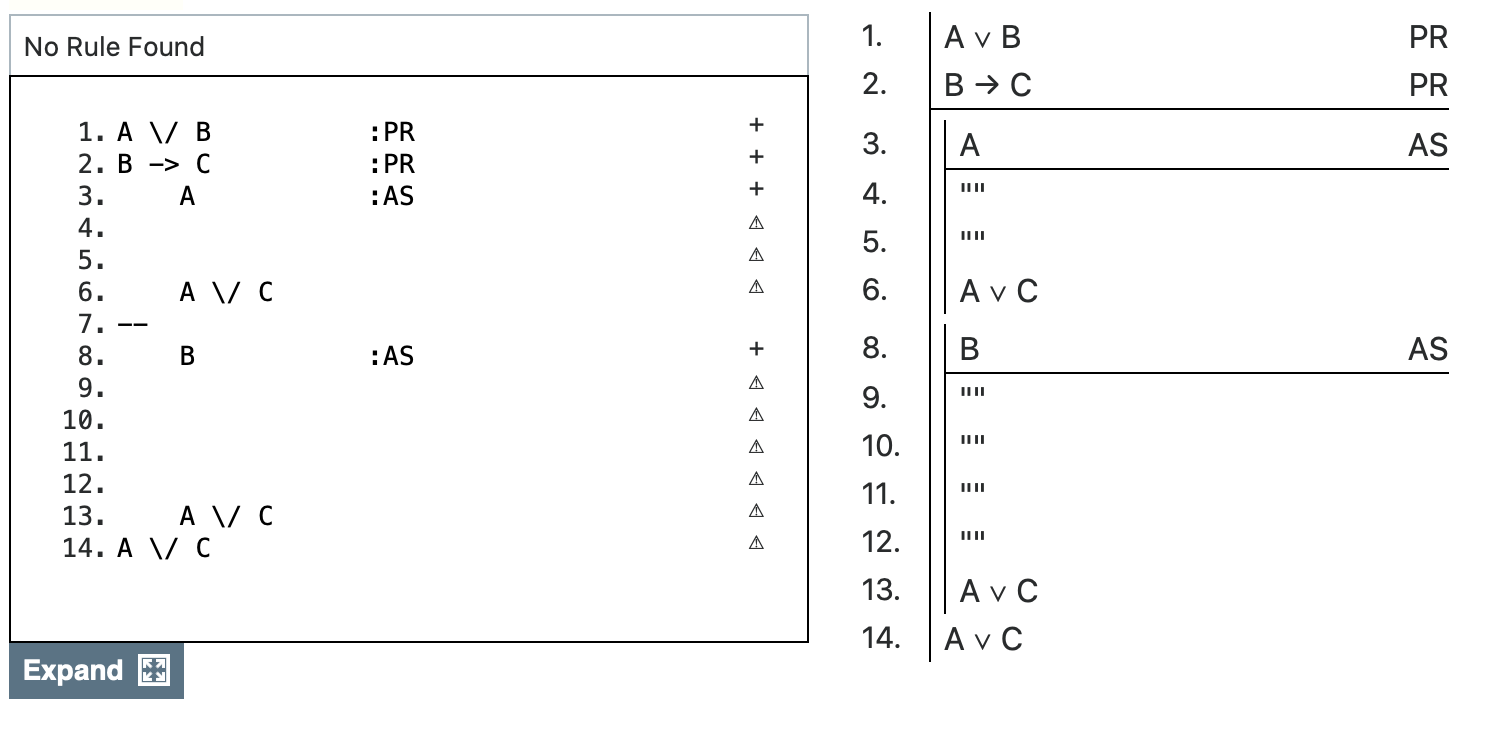
\includegraphics[width=\textwidth,height=0.75\textheight]{5_5b.png}
\caption{There are indents on all the blank lines}
\end{figure}
\end{frame}

\begin{frame}{\(A \vee B, B \rightarrow C \vdash A \vee C\)}
\protect\hypertarget{a-vee-b-b-rightarrow-c-vdash-a-vee-c-4}{}
\begin{figure}
\centering
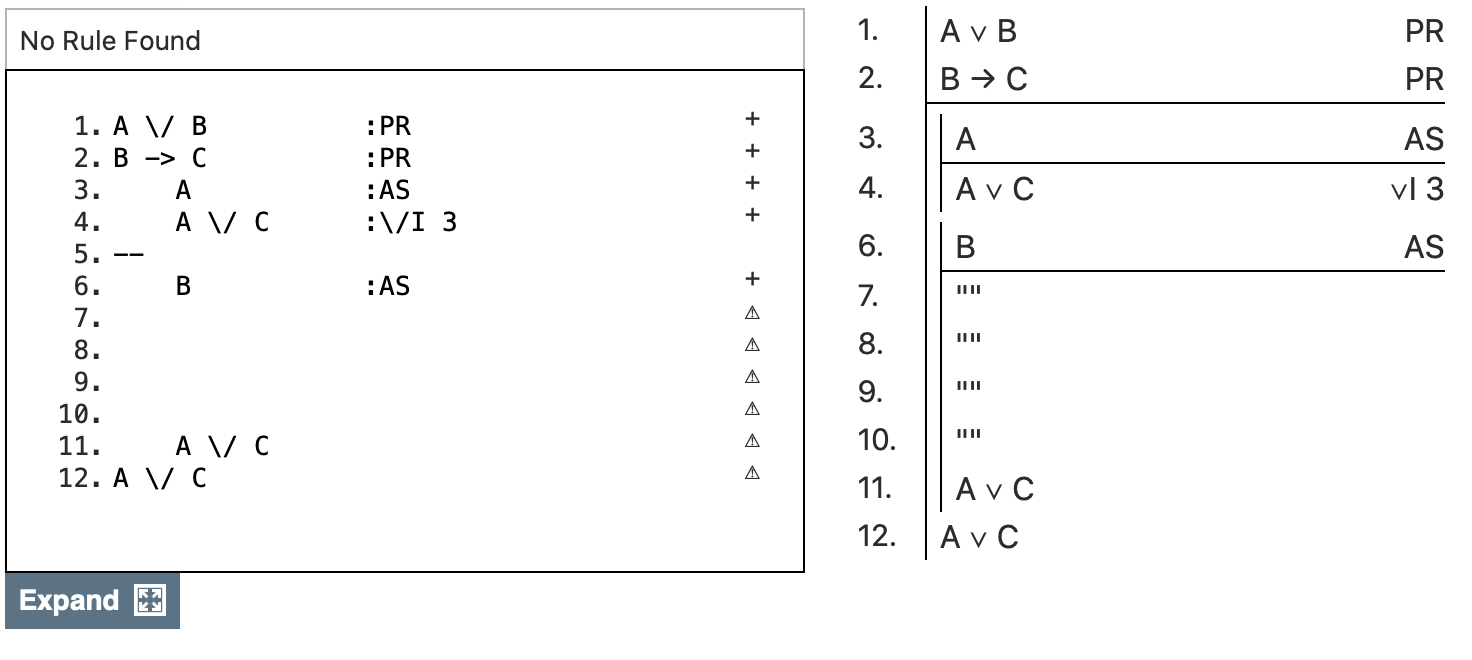
\includegraphics[width=\textwidth,height=0.75\textheight]{5_5c.png}
\caption{The left-hand subproof}
\end{figure}
\end{frame}

\begin{frame}{\(A \vee B, B \rightarrow C \vdash A \vee C\)}
\protect\hypertarget{a-vee-b-b-rightarrow-c-vdash-a-vee-c-5}{}
\begin{figure}
\centering
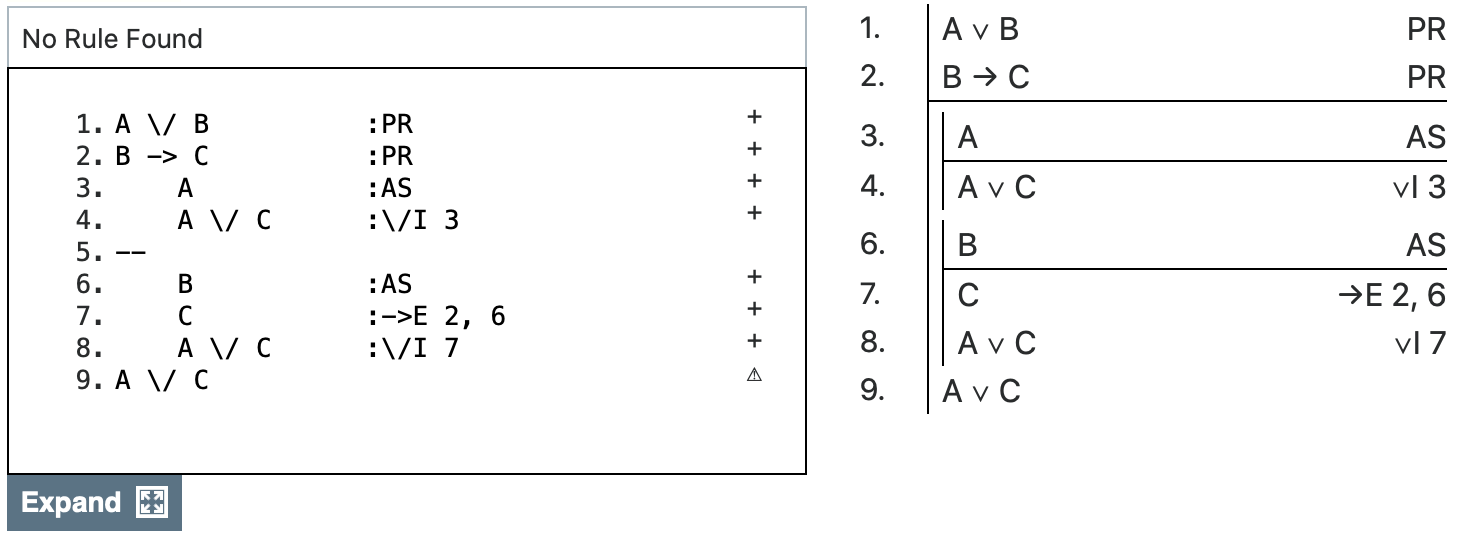
\includegraphics[width=\textwidth,height=0.75\textheight]{5_5d.png}
\caption{The right-hand subproof}
\end{figure}
\end{frame}

\begin{frame}{\(A \vee B, B \rightarrow C \vdash A \vee C\)}
\protect\hypertarget{a-vee-b-b-rightarrow-c-vdash-a-vee-c-6}{}
\begin{figure}
\centering
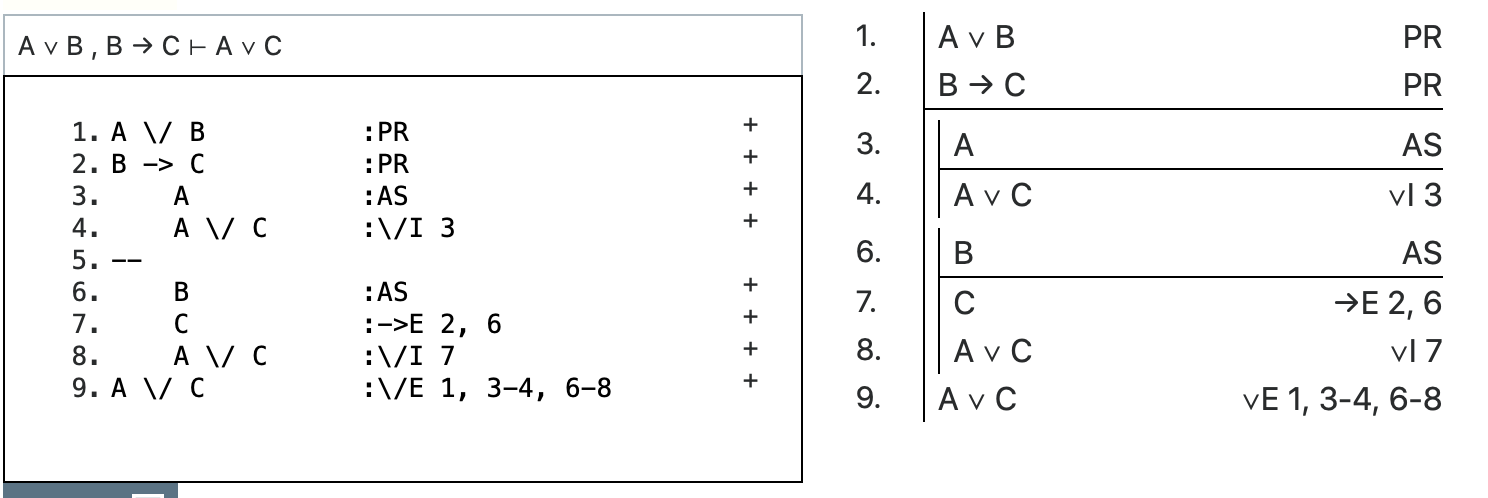
\includegraphics[width=\textwidth,height=0.75\textheight]{5_5e.png}
\caption{Finishing the proof - note the justifications}
\end{figure}
\end{frame}

\begin{frame}{Proofs From Disjunctions}
\protect\hypertarget{proofs-from-disjunctions}{}
\begin{itemize}
\tightlist
\item
  That's the basic structure.
\item
  They are a bit of a pain; I've illustrated almost the easiest one I
  could find.
\item
  But it's really important to keep track of what your goal is at every
  point.
\item
  For almost everyone, that's impossible if you try to just start at
  line 1 and work to line 9.
\item
  You have to bounce forward and backward in these proofs; just like
  I've done here.
\end{itemize}
\end{frame}

\begin{frame}{Working Forward from Not}
\protect\hypertarget{working-forward-from-not}{}
\begin{itemize}
\tightlist
\item
  It's going to be some kind of proof involving \(\bot\).
\item
  Whether that's Indirect Proof or \(\neg\)E isn't always clear, but
  that's going to be the structure.
\end{itemize}
\end{frame}

\begin{frame}{A Simple Strategy}
\protect\hypertarget{a-simple-strategy}{}
\begin{itemize}
\tightlist
\item
  If any of the premises is negated, then assume the opposite of the
  conclusion and try to derive \(\bot\).
\item
  If the conclusion is positive, its opposite is adding a negation.
\item
  If the conclusion is already negated, its opposite is deleting the
  negation.
\end{itemize}
\end{frame}

\begin{frame}{A More Complicated Strategy}
\protect\hypertarget{a-more-complicated-strategy}{}
\begin{itemize}
\tightlist
\item
  Sometimes the simple strategy won't be optimal.
\item
  Sometimes it will be quicker to do some working forward from the other
  premises, or backwards from the conclusion.
\item
  But the simple strategy is going to work, even in those cases.
\end{itemize}
\end{frame}

\begin{frame}{\(\neg A \vdash \neg (A \wedge B)\)}
\protect\hypertarget{neg-a-vdash-neg-a-wedge-b}{}
\begin{figure}
\centering
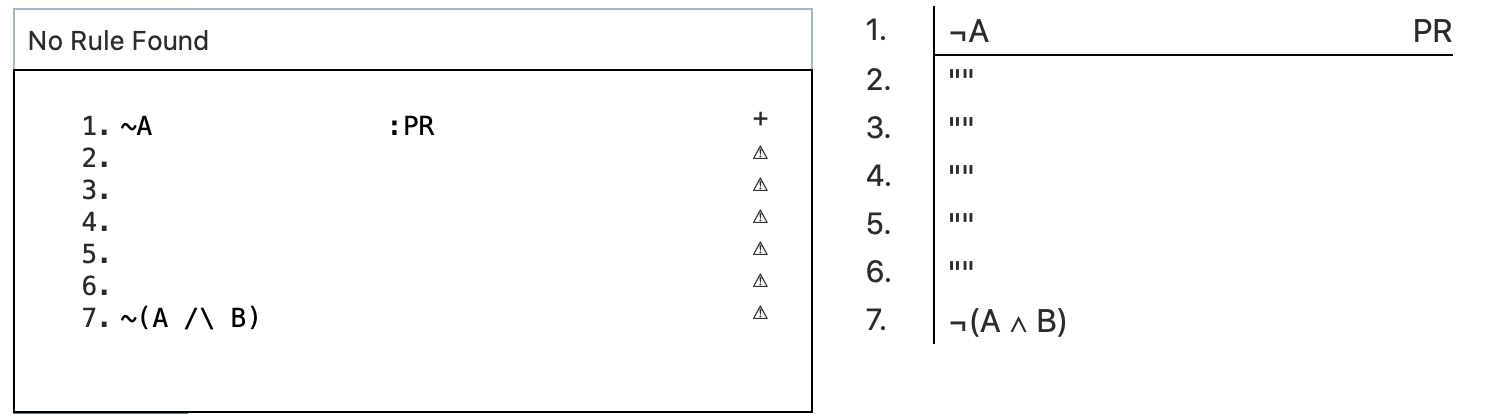
\includegraphics[width=\textwidth,height=0.75\textheight]{5_5f.png}
\caption{Premise and Conclusion}
\end{figure}
\end{frame}

\begin{frame}{\(\neg A \vdash \neg (A \wedge B)\)}
\protect\hypertarget{neg-a-vdash-neg-a-wedge-b-1}{}
\begin{figure}
\centering
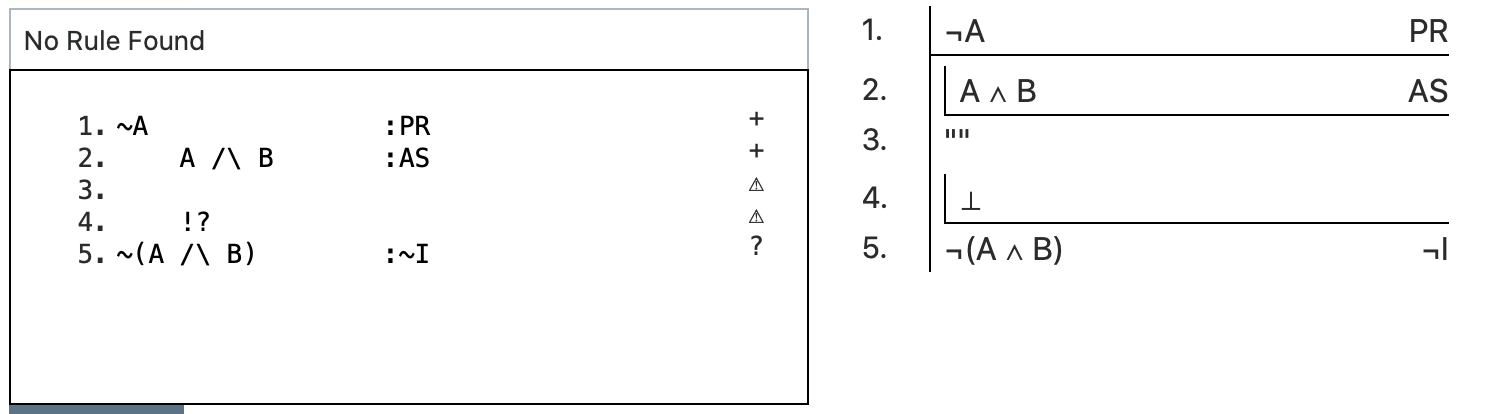
\includegraphics[width=\textwidth,height=0.75\textheight]{5_5g.png}
\caption{Set up \(\neg\)I - note how \(\bot\) is written}
\end{figure}
\end{frame}

\begin{frame}{\(\neg A \vdash \neg (A \wedge B)\)}
\protect\hypertarget{neg-a-vdash-neg-a-wedge-b-2}{}
\begin{figure}
\centering
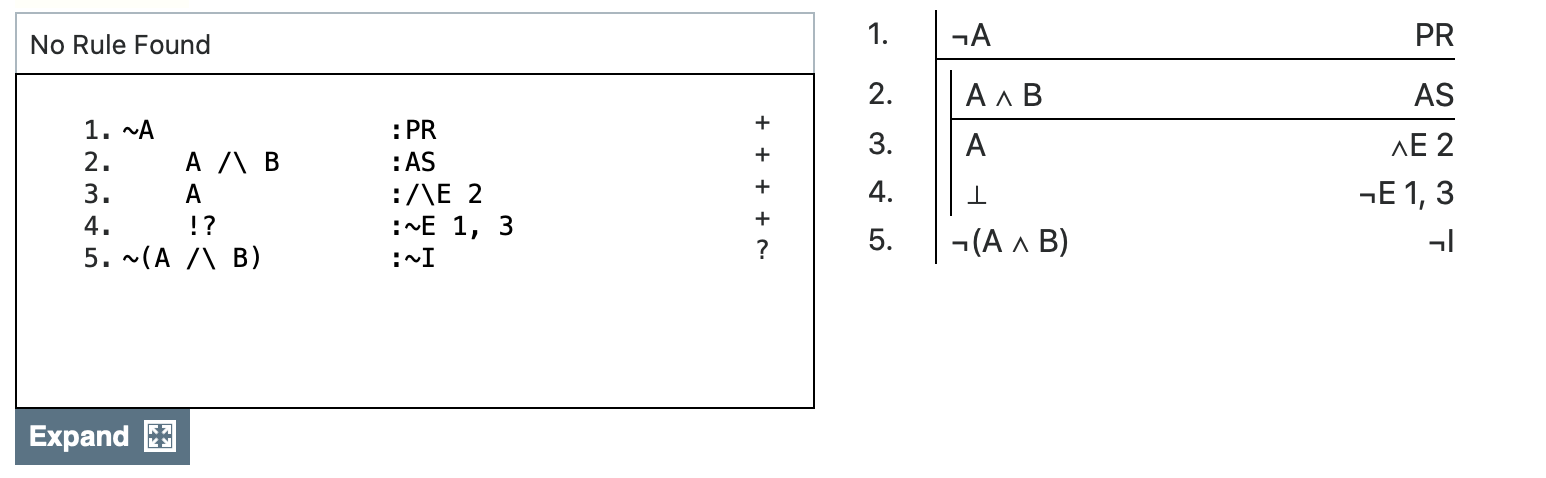
\includegraphics[width=\textwidth,height=0.75\textheight]{5_5h.png}
\caption{Derive the contradiction}
\end{figure}
\end{frame}

\begin{frame}{\(\neg A \vdash \neg (A \wedge B)\)}
\protect\hypertarget{neg-a-vdash-neg-a-wedge-b-3}{}
\begin{figure}
\centering
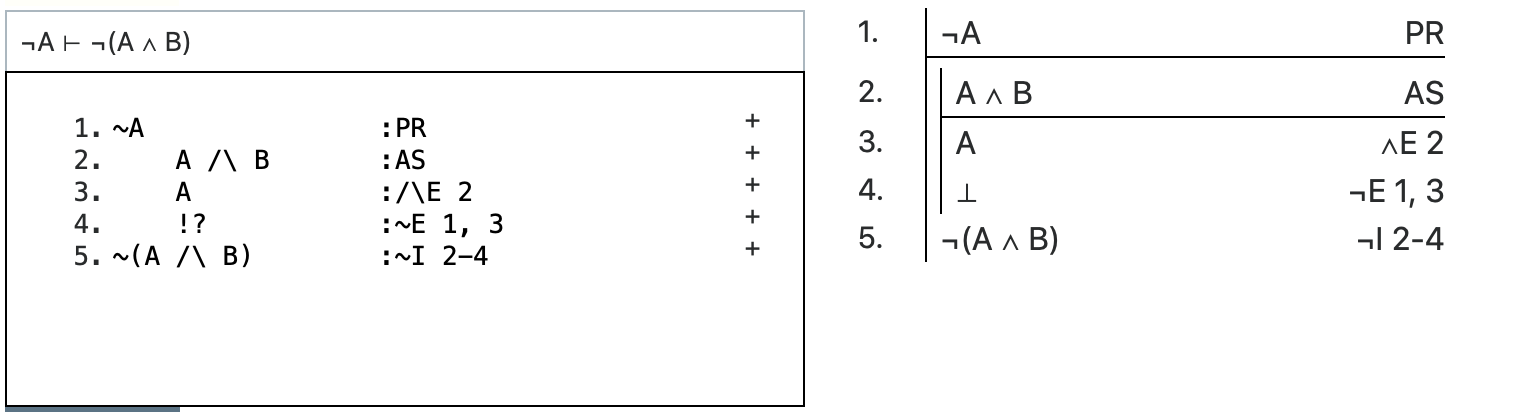
\includegraphics[width=\textwidth,height=0.75\textheight]{5_5i.png}
\caption{Finish the proof}
\end{figure}
\end{frame}

\begin{frame}{For Next Time}
\protect\hypertarget{for-next-time}{}
\begin{itemize}
\tightlist
\item
  I'll end with two special techniques
\end{itemize}
\end{frame}

\end{document}
